\section{Inheritance \& Abstract Classes}

Nedarvning handler om at lave specialiserede udgaver af allerede eksisterende og mere generelle klasser. Eksempelvis Employee-Manager forholdet diskuteret i Horstmann kap. 6; alle Managers er Employees, men ikke alle Employees er Managers. Managers er specielle typer af Employees, som har ekstra "features".

\subsection{Superclass (generel) og subclass (specialiseret)}

\begin{itemize}
  \item "is-a" forhold: $<$subclass$>$ "is-a" $<$superclass$>$
  \begin{itemize}
    \item Java-keyword: \verb|extends|
    \item \verb|public class Manager extends Employee { ... }|
    \item En class som er erklæret \verb|final| kan ikke extendes
    \item Alle classes extender Object
  \end{itemize}

  \item Subclasses arver alle metoder og variable fra deres superclass
  \item Subclasses kan override deres superclass' metoder, dog ikke hvis de er erklæret \verb|final|
  \begin{itemize}
    \item Polymorfi bestemmer hvilken metode der kaldes vha. objektets aktuelle type. En Employee variabel kan fx indeholde et Manager objekt (Liskov's substitutionsprincip\footnote{Liskov's substitutionsprincip siger, at et object af en subclass kan benyttes nårsomhelst et objekt af dens superclass forventes. Eksempelvis kan et Manager objekt altid tildeles en Employee variabel, men ikke den anden vej rundt. Da Manager objekter altid er garanteret at have samme metoder og variable (og lidt til) som Employee objekter, er dette netop muligt.}), og polymorfien sørger for at kalde Manager-objektets overridden metode - hvis en sådan eksisterer.
    \item Override-metoder skal have samme metodesignatur (samme return type, samme parametre), som superclassen's metode.
    \item Selvom en metode er overridden kan subclasses godt kalde deres superclass' version af metoden med keywordet \verb|super|.
    \item Preconditions til overridden metoder må ikke være mere strikse end superclassens preconditions. Hvis ingen preconditions findes i superclassen må subclassens overridden metode heller ikke have preconditions.
    \item Postconditions skal omvendt være mindst ligeså strikse.
    \item En overridden metode må ikke kaste yderligere check exceptions.
  \end{itemize}

  \item Subclasses kan kun tilgå private variable gennem \verb|get()| metoder, dog kan de tilgå protected variable (en slags "intern public")
  \item Nedarvning af classes betyder, at metoder og funktionalitet er tilgængelige med det samme, og principielt behøver man ikke skrive noget yderligere kode for at bruge sin nye subclass. Implementering (\verb|implements|) af interfaces betyder derimod, at man selv skal supplere koden for hver af de metoder, som interfacet definerer.
\end{itemize}

\subsection{Abstract classes}

\begin{itemize}
  \item Abstract classes er ikke instansiérbare - dvs. man kan ikke lave objekter af abstract classes. En class tagges som abstract med keywordet \verb|abstract|.\\
  Fx: \verb|public abstract class SelectableShape implements SceneShape|
  \begin{itemize}
    \item Eksempel: SelectableShape. Abstract class der implementerer SceneShape interfacet, og som definerer nogle af interfacets metoder, men ikke alle. De metoder som ikke er definerede skal derfor defineres i subclasses (fx CarShape, HouseShape).
    \item Abstract classes implementerer typisk noget af funktionaliteten i de interfaces de evt. implementerer, men ikke alt. Resten af metoderne er abstract.
    \item Fordele: Man kan lægge al ensartet funktionalitet for flere classes i én superclass, som implementerer et interface, som er nyttigt for disse classes.
    \item Ulemper: Classes kan kun extende én superclass, men implementere adskillige interfaces.
  \end{itemize}
  
  \item Refactoring - at omskrive kode så det er "bedre" eller lettere at forstå.\\
  Fx: "Extract superclass" - Lav en superclass ud fra de fælles features to eller flere classes har.
  
  \begin{center}
    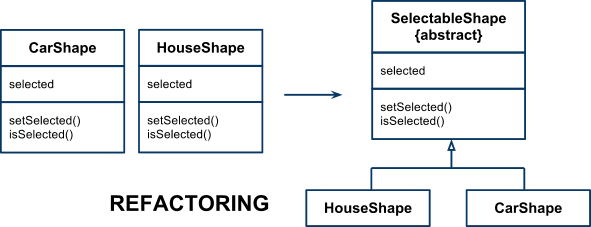
\includegraphics[scale=0.6]{images/refactor_to_template_method_pattern.png}
  \end{center}

  \begin{itemize}
    \item Refactoring adskiller sig fra design patterns idet refactoring handler om at omskrive allerede eksisterende kode, mens design patterns handler om at planlægge sit arbejde så man kan undgå at skulle benytte sig af refactoring.
  \end{itemize}

  \item Template method - en metode som flyttes fra subclasses til en superclass, og som kalder primitive operations, som kan være forskellige, i subclasses.
  \begin{itemize}
    \item Design pattern
    \item En \verb|templateMethod()| er en metode i en abstract class, som kalder abstract methods (dvs metoder som bliver defineret af subclasses som extender denne abstract class). Altså er en \verb|templateMethod()| en metode, som kalder andre metoder, som ikke endnu er blevet defineret.
    \item Eksempel: \verb|drawSelection()| i SelectableShape - \verb|drawSelection()| er defineret i SelectableShape, men kalder metoder \verb|draw()| og \verb|translate()|, som er abstract methods i SelectableShape, men som bliver defineret i CarShape og HouseShape.
  \end{itemize}

  \begin{center}
    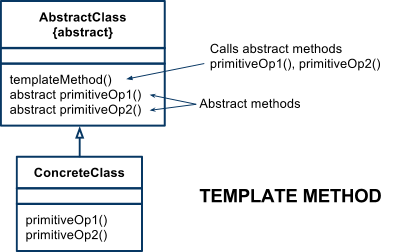
\includegraphics[scale=0.7]{images/template_method_pattern.png}
  \end{center}

  \item Protected interfaces
  \begin{itemize}
    \item protected er en mellemting mellem public og private; kan ses som "internt public" for alle subclasses til en class, men "eksternt private" for alle andre classes.
    \item Metoder kan kun bruge protected metoder/fields fra objekter af samme class som de ligger i. Fx kan HouseShape ikke kalde \verb|add()| på en CarShape, selvom de begge extender CompoundShape, som har en protected \verb|add()| metode.
    \item Protected fields bør undgås af samme grund som public fields bør undgås.
  \end{itemize}
\end{itemize}

\subsection{Hvornår er nedarvning ikke en god ide?}

\begin{itemize}
  \item Nedarvning bruges til "is-a" forhold.
  \begin{itemize}
    \item "is-a" forhold betyder at en class er en specialiseret version af en anden class. \\
Fx, "CarShape" is a "SelectableShape"
  \end{itemize}
  
  \item Aggregering bruges til "has-a" forhold.
  \begin{itemize}
    \item "has-a" forhold betyder at en class har et field hvis type er en anden class. \\
Fx, "Circle" has a "Point" - Circle classen har et Point objekt som sit centrum. Den er ikke et Point objekt i sig selv.
  \end{itemize}
  
  \item Nedarvning bør ikke bruges, hvis resultatet bryder med Liskov's substitutionsprincip.
Fx, \verb|Stack<T> extends Vector<T>| er en dum idé, da en stack og en vektor ikke har
noget med hinanden at gøre. Med en stack kan man kun push og pop elementer på
og af, og i LIFO\footnote{LIFO = Last In First Out} orden. Med en vektor kan man fjerne elementer tilfældige steder i arrayet.
\end{itemize}

